\documentclass[conference]{IEEEtran}
\IEEEoverridecommandlockouts
% The preceding line is only needed to identify funding in the first footnote. If that is unneeded, please comment it out.
\usepackage{cite}
\usepackage[spanish]{babel}
\usepackage{amsmath,amssymb,amsfonts}
\usepackage{algorithmic}
\usepackage{graphicx}
\usepackage{textcomp}
\usepackage{xcolor}
\def\BibTeX{{\rm B\kern-.05em{\sc i\kern-.025em b}\kern-.08em
    T\kern-.1667em\lower.7ex\hbox{E}\kern-.125emX}}
\graphicspath{ {images/} }
\renewcommand{\spanishtablename}{Tabla}%renombrar tablas en español%
\begin{document}

\title{Practica 1 \\ Predicción de rendimiento de gasolina en millas por galón de un auto mediante técnicas de regresión}

\author{\IEEEauthorblockN{1\textsuperscript{st} Erick Franco Gaona}
\IEEEauthorblockA{\textit{Departamento de Estudios Multidisciplinarios} \\
\textit{Universidad de Guanajuato}\\
Yuriria, México \\
e.francogaona@ugto.mx}
}

\maketitle

\begin{abstract}
This document is a model and instructions for \LaTeX.
This and the IEEEtran.cls file define the components of your paper [title, text, heads, etc.]. *CRITICAL: Do Not Use Symbols, Special Characters, Footnotes, 
or Math in Paper Title or Abstract.
\end{abstract}

\section{Introducción}

El análisis de regresión se usa ampliamente para hacer predicciones y estimaciones de expectativas condicionales de variables dependientes e independientes, y sus aplicaciones se superponen con el campo del aprendizaje automático. Ejecutar regresiones permite determinar los factores más importantes, los factores que a menudo se pasan por alto y cómo se influyen entre sí. Estos factores se denominan variables y se clasifican de la siguiente manera: \\

\begin{itemize}
\item Variable dependiente: Es el factor el cual se está tratando de entender o predecir (Y).
\item Variable(s) independiente(s): Es el factor que se cree que puede impactar en la variable dependiente (X). \\
\end{itemize}

Debido a eso la regresión suele usarse en las organizaciones ya que puede interpretar fenómenos y hacer predicciones sobre el futuro, así como obtener información empresarial valiosa y procesable. Este método proporciona información sobre cómo la estructura de costos y las características variables afectan el producto. Realizar análisis de regresión permite tomar decisiones comerciales más informadas y eficientes y desarrollar estrategias para mejorar la calidad de sus productos y servicios, lo que beneficia a su organización.

La figura 1 muestra cómo se relaciona el salario con los años de experiencia, prediciendo el salario de un trabajador dado. La regresión muestra una relación lineal positiva entre el salario (eje y) y los años de experiencia (eje x). Puede utilizar estos datos históricos para realizar previsiones salariales. En este trabajo se presentan dos metodos para realizar regresiones y se compara la efectividad de ambos aplicados para la predicción del rendimiento de la gasolina en millas por galón tomando un conjunto de datos público (mpg-auto) de diversos autos.

\begin{figure}[h]
    \centering
    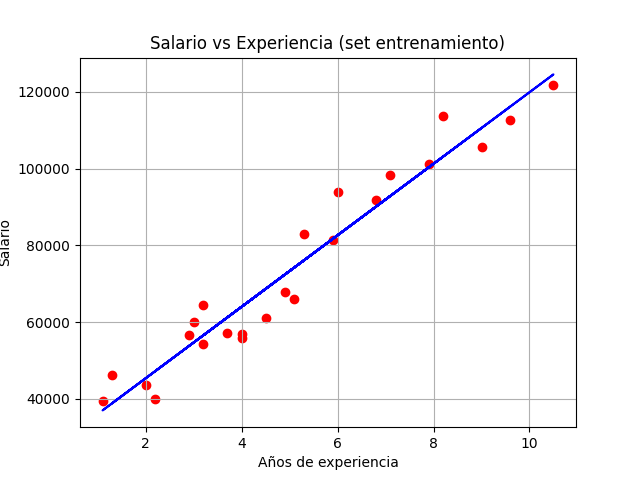
\includegraphics[scale=0.6]{1.png}
    \caption{Ejemplo de regresión aplicado en el salario vs los años de experiencia.}
    \label{fig:mesh1}
\end{figure}

\section{Teoría}
\subsection{Regresión lineal simple}
El análisis de regresión lineal simple se utiliza para predecir el valor de una variable en función del valor de otra variable. La regresión lineal se ajusta a una línea recta o a una superficie que minimiza las diferencias entre los valores de salida y los reales. Una forma razonable de relación entre la respuesta Y y el regresor x es la relación lineal

\begin{equation}
Y= \beta_0 + \beta_1x
\end{equation}

en la que, $\beta_0$ es la intersección de la recta y $\beta_1$ es la pendiente.\\

Si la relación es exacta y no contiene componentes aleatorios o probabilísticos, se trata de una relación determinista entre dos variables. Sin embargo, en muchos casos reales, la relación no es determinista, es decir, una x dada no siempre produce el mismo valor de Y. Debido a esa situación, los problemas son de naturaleza probabilística, toda vez que la relación anterior no puede considerarse exacta. El concepto de análisis de regresión se refiere a encontrar la mejor relación entre Y y x cuantificando la fuerza de esa relación, y empleando métodos que permitan predecir los valores de la respuesta dados los valores del regresor x. En resumen la regresión lineal simple, trata el caso de una sola variable regresora, en el que la relación entre x y y es lineal.\\

El método de los mínimos cuadrados se utiliza para calcular la recta de regresión lineal que minimiza los residuos, es decir, las diferencias entre los valores reales y los estimados por la recta. Con este método se debe calcular $b_0$ y $b_1$, los estimados de $\beta_0$ y $\beta_1$, de manera que la suma de los cuadrados de los residuales sea mínima. Los estimados $b_0$ y $b_1$ de los mínimos cuadrados de los coeficientes de regresión $\beta_0$ y $\beta_1$ se calculan mediante las fórmulas

\begin{equation}
b_1= \frac{\sum_{i=1}^{n}(x_i-\bar{x})(y_i-\bar{y})}{\sum_{i=1}^{n}(x_i-\bar{x})^{2}}
\end{equation}

\begin{equation}
b_0= \frac{\sum_{i=1}^{n} y_i - b_1 \sum_{i=1}^{n}x_i}{n}
\end{equation}

\subsection{Regresión lineal multiple}
En muchas aplicaciones habrá más de un regresor, es decir, más de una variable independiente que ayude a explicar a Y. Por ejemplo, si se tratara de un problema con dos regresores la estructura múltiple de la regresión se podría escribir como

\begin{equation}
Y= \beta_0 + \beta_1x_1 + \beta_2x_2
\end{equation}

el modelo de regresión lineal múltiple general se expresa de la siguiente manera 


\begin{equation}
Y= \beta_0 + \beta_1x_1 + ... + \beta_kx_k
\end{equation}

donde cada coeficiente de regresión $\beta_i$ se estima por medio de $b_i$, a partir de los datos muestrales, usando el método de mínimos cuadrados. Si se acomoda en forma matricial se tiene que:

\begin{equation}
\begin{pmatrix}
y_1 \\
y_2 \\
\vdots \\
y_n 
\end{pmatrix}
=
\begin{pmatrix}
1 & x_{11} & \dotsi x_{k1}\\
1 & x_{12} & \dotsi x_{k2}\\
1 & n & \dotsi x_{kn}
\end{pmatrix}
\begin{pmatrix}
\beta_0 \\
\beta_1 \\
\vdots \\
\beta_k
\end{pmatrix}
+
\begin{pmatrix}
\epsilon_0 \\
\epsilon_1 \\
\vdots \\
\epsilon_n
\end{pmatrix}
\end{equation}

\begin{equation}
Y=X\beta+\epsilon
\end{equation}

Para encontrar las $\beta$ se tiene de forma matricial que
\begin{equation}
\beta=(X^TX)^{-1}X^TY
\end{equation}
\section{Resultados}
Before you begin to format your paper, first write and save the content as a 
separate text file. Complete all content and organizational editing before 
formatting. Please note sections \ref{AA}--\ref{SCM} below for more information on 
proofreading, spelling and grammar.

Keep your text and graphic files separate until after the text has been 
formatted and styled. Do not number text heads---{\LaTeX} will do that 
for you.

\section*{Conclusiones}

The preferred spelling of the word ``acknowledgment'' in America is without 
an ``e'' after the ``g''. Avoid the stilted expression ``one of us (R. B. 
G.) thanks $\ldots$''. Instead, try ``R. B. G. thanks$\ldots$''. Put sponsor 
acknowledgments in the unnumbered footnote on the first page.

\section*{Referencias}

Please number citations consecutively within brackets \cite{b1}. The 
sentence punctuation follows the bracket \cite{b2}. Refer simply to the reference 
number, as in \cite{b3}---do not use ``Ref. \cite{b3}'' or ``reference \cite{b3}'' except at 
the beginning of a sentence: ``Reference \cite{b3} was the first $\ldots$''

Number footnotes separately in superscripts. Place the actual footnote at 
the bottom of the column in which it was cited. Do not put footnotes in the 
abstract or reference list. Use letters for table footnotes.

Unless there are six authors or more give all authors' names; do not use 
``et al.''. Papers that have not been published, even if they have been 
submitted for publication, should be cited as ``unpublished'' \cite{b4}. Papers 
that have been accepted for publication should be cited as ``in press'' \cite{b5}. 
Capitalize only the first word in a paper title, except for proper nouns and 
element symbols.

For papers published in translation journals, please give the English 
citation first, followed by the original foreign-language citation \cite{b6}.


\begin{thebibliography}{00}
\bibitem{b1} G. Eason, B. Noble, and I. N. Sneddon, ``On certain integrals of Lipschitz-Hankel type involving products of Bessel functions,'' Phil. Trans. Roy. Soc. London, vol. A247, pp. 529--551, April 1955.
\bibitem{b2} J. Clerk Maxwell, A Treatise on Electricity and Magnetism, 3rd ed., vol. 2. Oxford: Clarendon, 1892, pp.68--73.
\bibitem{b3} I. S. Jacobs and C. P. Bean, ``Fine particles, thin films and exchange anisotropy,'' in Magnetism, vol. III, G. T. Rado and H. Suhl, Eds. New York: Academic, 1963, pp. 271--350.
\bibitem{b4} K. Elissa, ``Title of paper if known,'' unpublished.
\bibitem{b5} R. Nicole, ``Title of paper with only first word capitalized,'' J. Name Stand. Abbrev., in press.
\bibitem{b6} Y. Yorozu, M. Hirano, K. Oka, and Y. Tagawa, ``Electron spectroscopy studies on magneto-optical media and plastic substrate interface,'' IEEE Transl. J. Magn. Japan, vol. 2, pp. 740--741, August 1987 [Digests 9th Annual Conf. Magnetics Japan, p. 301, 1982].
\bibitem{b7} M. Young, The Technical Writer's Handbook. Mill Valley, CA: University Science, 1989.
\end{thebibliography}
\vspace{12pt}
\color{red}
IEEE conference templates contain guidance text for composing and formatting conference papers. Please ensure that all template text is removed from your conference paper prior to submission to the conference. Failure to remove the template text from your paper may result in your paper not being published.

\end{document}